\section{Design} \mdseries 
BrainGrid has undergone recent refactoring and data reorganization due to a need to simplify the implementations of other models. The original legacy code was formatted in an object-oriented fashion, with the multiple simulator/network objects branching out into a complicated list of files and methods that made implementing additional incredibly complex, as implementing said model would require modifying half-a-dozen files and much of these changes would end up being redundant. 
\begin{figure}
	\centering
		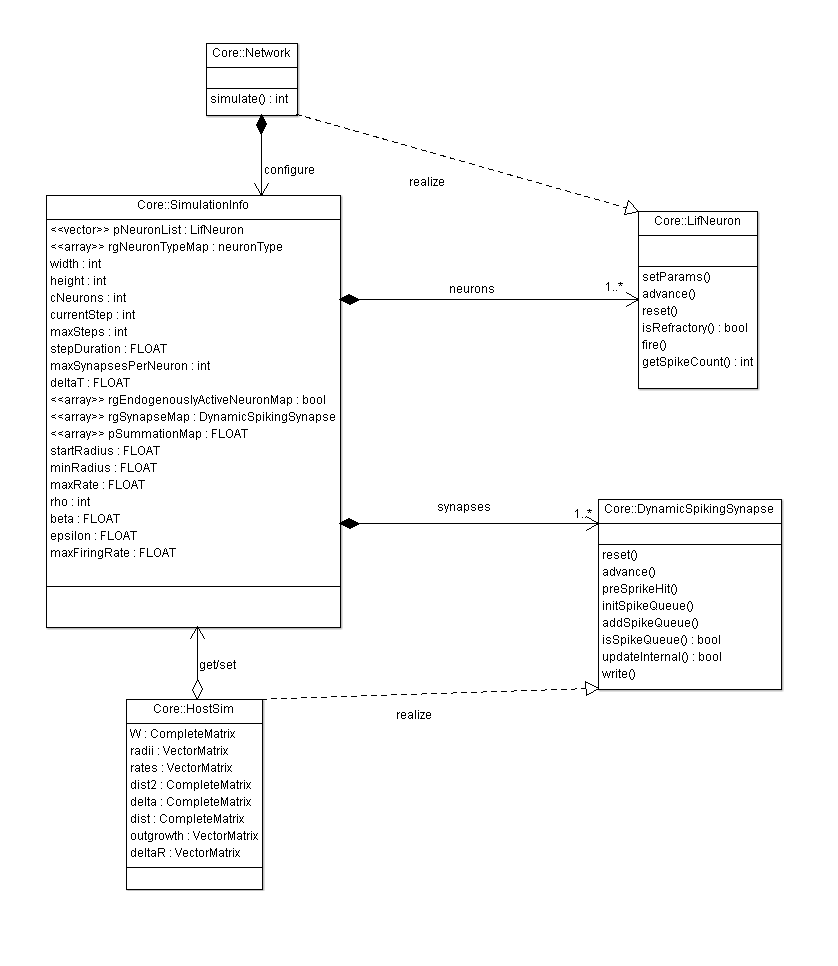
\includegraphics[width=.6\textwidth]{./diagrams/OldDiagram.png}
		\caption{BrainGrid's old design}
\end{figure}
\pagebreak

\noindent \mdseries The refactoring process of BrainGrid reorganized the data structures of the legacy code in order to implement a simpler program structure that prioritizes separating the model-dependent code from the model independent. The new code also stripped away some of the object-oriented structure of the neurons and the synapses, and instead now uses a data-centric structure, which utilizes two different structs as the containers of all neuron and synapse data. This structure was originally designed for the GPU implementation of the simulator, and this refactored version of the simulator simply uses that design for all other implementations as well. This is to simplify transitioning from single-threaded to multi-threaded.

\begin{figure}
	\centering
		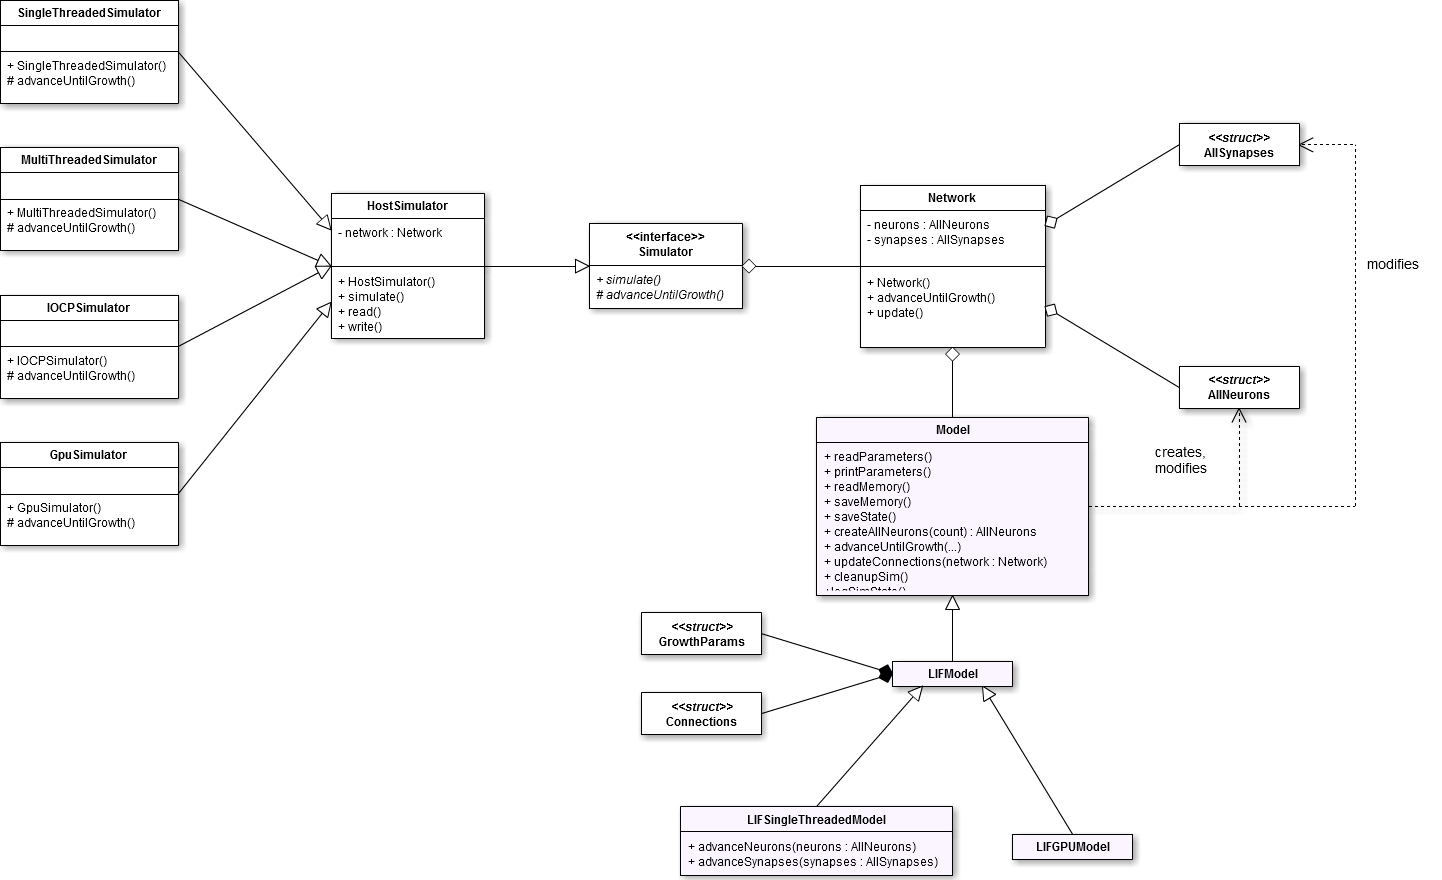
\includegraphics[width=\textwidth]{./diagrams/NewDiagram.png}
		\caption{BrainGrid's new design}
\end{figure}
\pagebreak
